\section{Data preprocessing}

\subsection{Resizing and Normalization}
Before applying the classification models we preprocessed our image data. We started off by resizing each image to a window of pixels of \(64 \times 64\), forming a square. Although all the images had the same size before this step, we decided to resize them to a base size that would form a square because it's usually standard procedure in face detection problems.

After this step we validated that each image was in gray-scale, converting from RGB to GRAY and making the problem less complex by having only one dimension to analyze instead of three. We also applied Adaptive Histogram Equalization in the images, so that contrast and luminosity effects were reduced, following the advice and procedure of the authors of the paper \cite{609310}.

To finalize the preprocessing phase, we normalized each image by dividing the pixel values by 255 achieving consistency in all our images, with the pixel values ranging from zero to one.

\subsection{Data Augmentation}
As we stated in section \ref{data-visualization}, the dataset we were given had a total of 124 images. This is an incredibly small dataset and we weren't able to achieve satisfactory results with it, so, we decided to expand the dataset with data augmentation, following some of the practices showcased by the research work explained in \cite{8858529}.

Considering the slight imbalance between the number of examples of face images and non-face images we adopted the following strategy:

\begin{itemize} 
\item Each face image produces 3 new images through reflection and dislocation.
\item Each non-face image produces 4 new images through reflection, dislocation and by inserting a random level of noise.
\end{itemize}

Thereby, ending up with a total of 551 images, 276  of  which  are  face images and 275 are non-face images.

\subsection{Histogram of oriented gradients}
The Histogram of Oriented Gradients (HOG) is a feature descriptor used in computer vision, more specifically in the field of object detection. Instead of our algorithm analysing each image,pixel by pixel, the HOG will count occurrences of gradient orientation in localized portions of an image, improving it's performance. 
Our implementation was based on the example documented in \cite{scikit-hog}, provided by the scikit-image documentation.

\begin{figure}[htbp]
\centerline{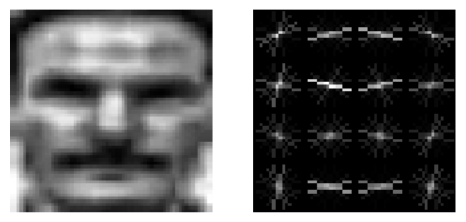
\includegraphics[scale=0.35]{images/hog_image.png}}
\caption{HOG feature extraction}
\label{fig:hog}
\end{figure}

Figure \ref{fig:hog} shows an example of an image before and after applying the Histogram of Oriented Gradients extraction.